% !TeX spellcheck = de_DE
\documentclass[a4paper,11pt]{ctexart}

\usepackage{setspace}
\usepackage{titlesec}
\usepackage{titletoc}
\usepackage[shortlabels]{enumitem}
\usepackage[hmargin=1.25in,vmargin=1in]{geometry}
\usepackage{amsmath}
\usepackage{amssymb}
\usepackage{indentfirst}
\usepackage[colorlinks,linkcolor=blue,anchorcolor=blue,citecolor=green]{hyperref}
\usepackage{tikz}
\usetikzlibrary{arrows.meta}
\usetikzlibrary{bending}
\usetikzlibrary{math}
\usetikzlibrary{shapes.symbols}
\usetikzlibrary{shapes.geometric}
\usetikzlibrary{shapes.arrows}
\usepackage[american inductors]{circuitikz}
\usepackage{booktabs}
\usepackage{array}
\usepackage{multirow}
\usepackage{upgreek}
\usepackage{xfrac}
\usepackage{subfig}
\usepackage{float}
\usepackage{placeins}
\usepackage{url}
\usepackage{lscape}
\usepackage{rotating}
\usepackage{graphicx}
\graphicspath{{screen/}}
\usepackage{pythonhighlight}

\renewcommand\theequation{\arabic{equation}}
\renewcommand{\contentsname}{}
\renewcommand\arraystretch{1.5}

\newcommand{\kV}{\,\text{kV}}
\newcommand{\V}{\,\text{V}}
\newcommand{\Ohm}{\,\Omega}
\newcommand{\MOhm}{\,M\Omega}
\renewcommand{\H}{\,\text{H}}
\newcommand{\s}{\,\text{s}}
\newcommand{\kA}{\,\text{kA}}
\newcommand{\A}{\,\text{A}}
\newcommand{\MW}{\,\text{MW}}
\newcommand{\W}{\,\text{W}}
\newcommand{\MVar}{\,\text{MVar}}
\newcommand{\MVA}{\,\text{MVA}}
\renewcommand{\S}{\,\text{S}}
\newcommand{\km}{\,\text{km}}
\newcommand{\diff}{\text{d}}
\newcommand{\Hz}{\,\text{Hz}}
\newcommand{\kHz}{\,\text{kHz}}
\renewcommand{\j}{\text{j}}
\newcommand{\ssum}{\scriptscriptstyle \sum}

%\renewcommand{\omega}{\upomega}

\newcommand{\du}[1]
{
	#1^{\circ}
}
\newcommand{\ang}[1]
{
	\angle#1^{\circ}
}

\newcommand{\bfem}[1]
{
	\em\bfseries#1\normalfont
}

\newcommand{\subpar}
{
	\par
	\hangafter = 0
	\setlength{\hangindent}{1em}
}

\newcommand{\subsubpar}
{
	\par
	\hangafter = 0
	\setlength{\hangindent}{2em}
}
\newcommand{\subsubsubpar}
{
	\par
	\hangafter = 0
	\setlength{\hangindent}{3em}
}

\newcommand{\AuthorX}
{
	
	\zihao{-3}
	\hspace{2em}姓名\hspace{1em} \underline{\hspace{4em}谢弘洋\hspace{4em}}\\
	\vspace{1em}
	\hspace{2em}学号\hspace{1em} \underline{\hspace{2.5em}515021910641\hspace{2.5em}}\\
	\vspace{1em}
	同组姓名\hspace{1em} \underline{\hspace{2em}孟诗涵\hspace{1em}陈晓彤\hspace{2em}}\\
}

\newcommand{\AuthorM}
{
	
	\zihao{-3}
	\hspace{2em}姓名\hspace{1em} \underline{\hspace{4em}孟诗涵\hspace{4em}}\\
	\vspace{1em}
	\hspace{2em}学号\hspace{1em} \underline{\hspace{2.5em}515021910063\hspace{2.5em}}\\
	\vspace{1em}
	同组姓名\hspace{1em} \underline{\hspace{2em}谢弘洋\hspace{1em}陈晓彤\hspace{2em}}\\
}

\newcommand{\AuthorC}
{
	
	\zihao{-3}
	\hspace{2em}姓名\hspace{1em} \underline{\hspace{4em}陈晓彤\hspace{4em}}\\
	\vspace{1em}
	\hspace{2em}学号\hspace{1em} \underline{\hspace{2.5em}515021910659\hspace{2.5em}}\\
	\vspace{1em}
	同组姓名\hspace{1em} \underline{\hspace{2em}谢弘洋\hspace{1em}孟诗涵\hspace{2em}}\\
}

\newenvironment{shrinkeq}[2]
{
	\bgroup
	\addtolength\abovedisplayshortskip{#1}
	\addtolength\abovedisplayskip{#1}
	\addtolength\belowdisplayshortskip{#2}
	\addtolength\belowdisplayskip{#2}
}
{
	\egroup
	\ignorespacesafterend
}

\setcounter{secnumdepth}{4}

\title
{
	\linespread{1.5} \zihao{4}
	高压数字测量系统课程设计 \\ 
	\zihao{2}
	开题报告
}
\author
{
	谢弘洋
}
\date{}

\begin{document}
	\pagestyle{plain}

\begin{figure}[t]
	\setlength{\abovecaptionskip}{-10mm}
	\setlength{\belowcaptionskip}{-60mm}
	\centering
	
\includegraphics[scale=0.4]{page1.png}
\end{figure}

\begin{center}
	\zihao{-2}
	高\,压\,数\,字\,测\,量\,系\,统\,课\,程\,设\,计 \\
	\vspace{0.7em}
	
	\zihao{1}
	中\hspace{0.5em} 期\hspace{0.5em} 报\hspace{0.5em} 告\\
	\vspace{3em}
		
	\AuthorX
	
	\vspace{6em}
	\today
\end{center}

\titleformat{\section}{\Large\bfseries\raggedright}{\chinese{section}}{10pt}{}
\titlespacing{\section}{0pt}{10pt}{5pt}
\titleformat{\subsection}{\bfseries\zihao{-4}}{\arabic{subsection}.}{5pt}{}
\titlespacing{\subsection}{1em}{2pt}{3pt}
\titleformat{\subsubsection}{\bfseries\normalsize}{\arabic{subsection}.\arabic{subsubsection}}{5pt}{}
\titlespacing{\subsubsection}{2em}{1pt}{0pt}
\titleformat{\paragraph}{\bfseries\normalsize}{\arabic{subsection}.\arabic{subsubsection}.\arabic{paragraph}}{5pt}{}
\titlespacing{\paragraph}{3em}{1pt}{0pt}

\newpage
\begin{spacing}{1.5}

\zihao{-4}

\section{进度概述}
\par
在半个学期的时间里,小组成员利用课余时间,查阅资料、实践探索,在共同努力下使得项目进度稳步推进,目前已经完成的内容如下:
\begin{enumerate}[1.,topsep=0pt]
	\setlength{\itemsep}{-0.25\baselineskip}
	\item 搭建云服务器平台,安装及配置服务器框架、资源和端口。
	\item 云服务器程序的编写,实现了数据接收和进行简单处理的功能。
	\item 4G模块的调试和使用,能够通过串口实现和服务器的双向数据收发。
	\item 在PC端编写Python程序,实现串口数据发送和接收功能,为下一步大量数据点的发送和接收做好准备。
\end{enumerate}
\par
下面将对各个任务的具体内容以及小组成员所作工作进行简要叙述。

\section{云服务器搭建}
\subsection{云服务器的购买与登录}
\par
本小组选择腾讯云作为项目初期使用的云服务器平台,进入腾讯云官方网站(\url{https://cloud.tencent.com/}),绑定微信登录后,完成在校学生认证后即可以10元/月的价格购买指定的服务器套餐,并拥有两次续费机会(每次最长12个月)。在购买界面可以选择服务器操作系统,本小组选择了CentOS系统,作为Linux发行版之一,在网上能找到许多相关的资料和服务器搭建教程,方便学习与实践。
\begin{figure}[h]
	\centering
	\setlength{\abovecaptionskip}{2mm}
	\setlength{\belowcaptionskip}{-2mm}
	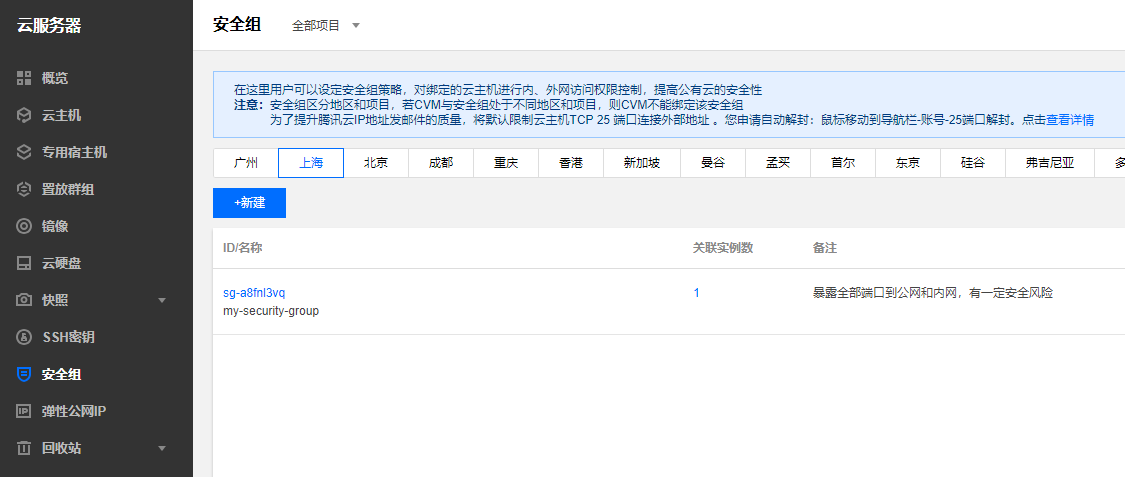
\includegraphics[scale=0.35]{安全组1.png}
	\caption{控制台安全组菜单}\label{figure:安全组1}
\end{figure}
\begin{figure}[h]
	\centering
	\setlength{\abovecaptionskip}{2mm}
	\setlength{\belowcaptionskip}{-2mm}
	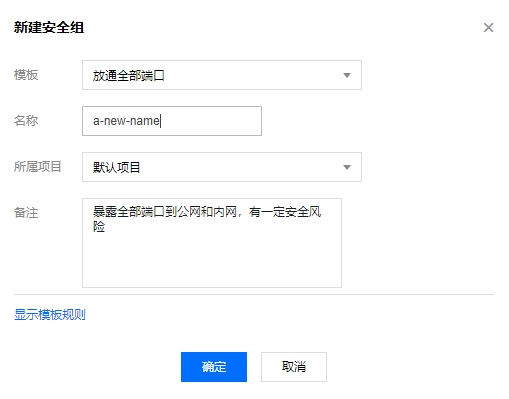
\includegraphics[scale=0.25]{安全组2.png}
	\caption{新建安全组}\label{figure:安全组2}
\end{figure}
\begin{figure}[h]
	\centering
	\setlength{\abovecaptionskip}{2mm}
	\setlength{\belowcaptionskip}{-2mm}
	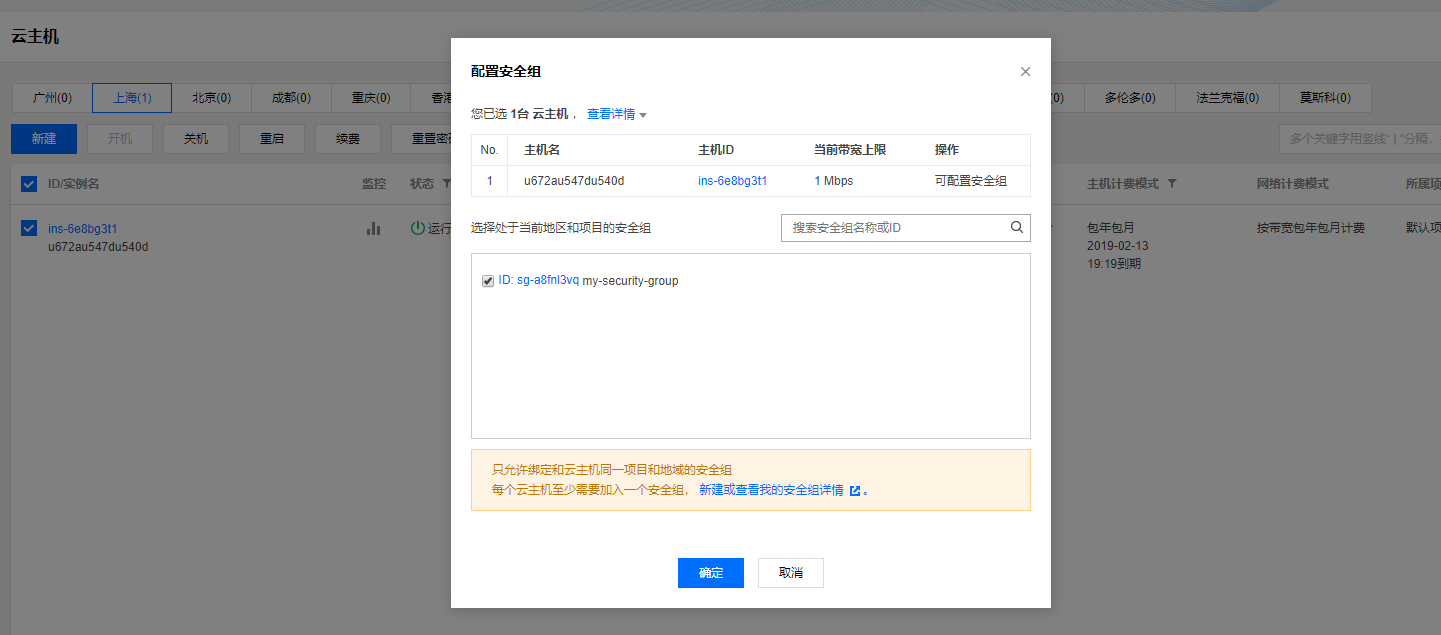
\includegraphics[scale=0.25]{安全组3.png}
	\caption{配置安全组}\label{figure:安全组3}
\end{figure}
\par
云服务器的正常使用需要首先为其配置安全组,在腾讯云服务器控制台界面进入左侧的安全组菜单,点击新建安全组,由于当前的云服务器仅作为学习探索使用,并没有重要资料,可以直接使用提供的“放通全部端口”的模板。完成安全组创建后,在云主机列表中,选择“更多”操作中的“安全组”-“配置安全组”,选择刚刚创建的安全组;也可以直接选择“安全组”-“一键放通”完成安全组的配置。完成安全组的配置后,即可以选择“登录”操作,初始用户名“root”(最终权限用户),填入购买服务器后收到的密码即可完成云服务器登录。由于初始密码往往复杂且无规律,可以从云主机列表的“更多”操作下选择“密码/密钥”-“重置密码”完成密码重置。
\begin{figure}[h]
	\centering
	\setlength{\abovecaptionskip}{2mm}
	\setlength{\belowcaptionskip}{-2mm}
	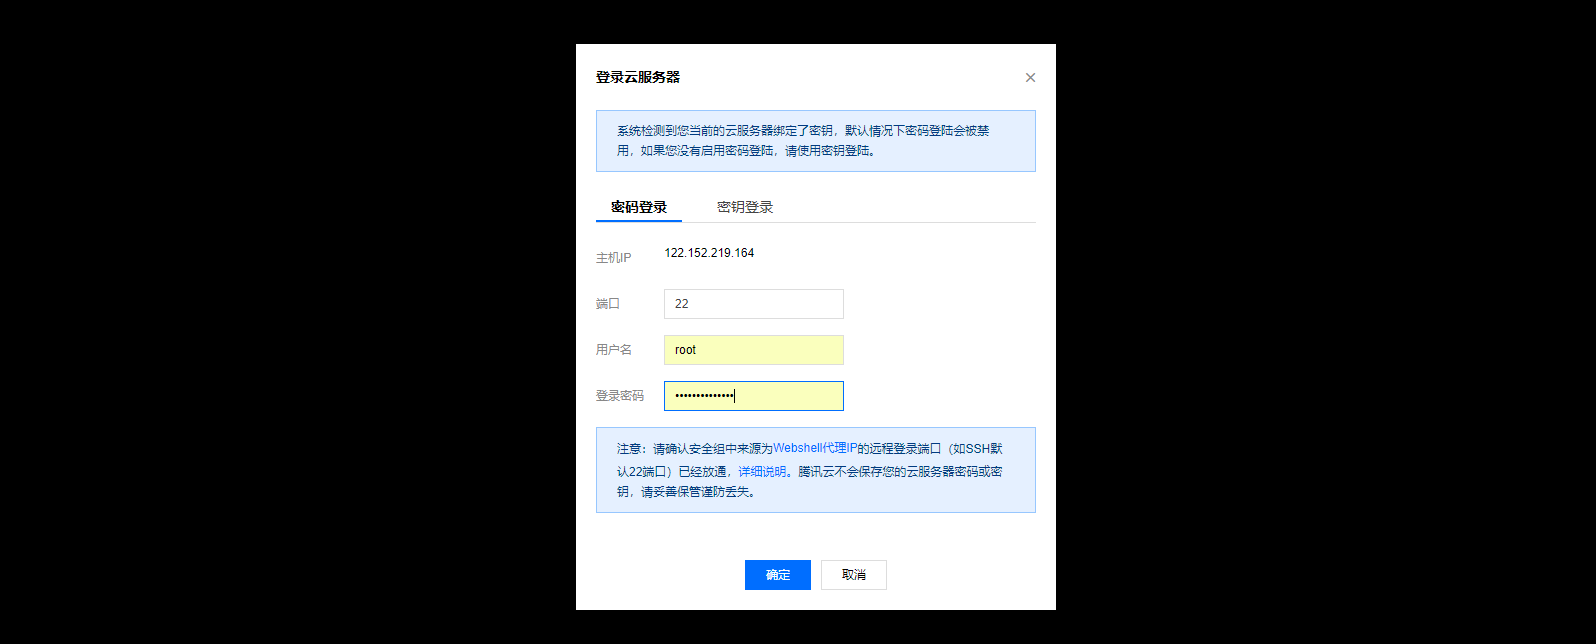
\includegraphics[scale=0.25]{登录1.png}
	\caption{登录云服务器}\label{figure:登录1}
\end{figure}
\subsection{使用SSH密钥登录云服务器}
\par
上述登录云服务器的操作以用户名和密码的方式,通过腾讯云提供的WebShell完成,而如果配置了SSH密钥,不仅可以更为快捷地完成登录操作,也能够通过各种远程登录工具(如PuTTY)实现云服务器的登录和相关操作。
\par
首先完成SSH密钥的创建和绑定,进入控制台左侧的SSH密钥菜单,新建密钥,选择“创建新密钥对”,并下载创建的密钥。之后,首先需要将正在运行的云主机关机,之后同样从“更多”操作中选择“密码/密钥”-“加载密钥”,选择之前创建的密钥名称,完成绑定。此时,再次选择登录操作,选择“密钥登录”,在“密钥文件”一栏选择之前下载的密钥文件,即可完成登录。
\par
而使用PuTTY登录云服务器首先需要下载PuTTY(\url{https://www.putty.org/})。完成安装后,首先运行PuTTYgen,选择“Conversions”-“Import Key”,加入之前下载的密钥文件后,点击“Save private Key”,保存私钥。之后,打开PuTTY,配置远程会话模板。在“Connection”-“Data”中的“Auto-login usename”一栏填入默认用户名“root”;在“Connection”-“SSH”-“Auth”中选择加入之前保存的私钥文件;最后,在“Session”中的“Host Name”中填入服务器的公网IP地址,端口选择22,并保存当前会话,之后即可以直接按照本次配置进行云服务器的登录。点击“Open”即可登录云服务器。
\subsection{云服务器端资源安装}
\subsubsection{Python安装}
\par
由于最新版本的Python和服务器操作系统的尚存在不少兼容性问题,因此选择安装较为成熟的Python3.6.4版本。首先进入希望的安装目录:
\begin{verbatim}
    cd ..
    cd usr/local
\end{verbatim}
之后下载Python安装包:
\begin{verbatim}
    wget https://www.python.org/ftp/python/3.6.4/Python-3.6.4.tgz
\end{verbatim}
解压安装包:
\begin{verbatim}
    tar -zxvf Python-3.6.4.tgz
\end{verbatim}
安装到指定位置(由第二条语句配置):
\begin{verbatim}
    cd Python-3.6.4
    ./configure --prefix=/usr/local/python3
    make && make install
\end{verbatim}
配置软连接(相当于环境变脸配置,由于CentOS已经安装了Python-2.7,因此需要将python命令关联到Python-3.6.4上):
\begin{verbatim}
     ln -s /usr/local/python3 /usr/bin/python
\end{verbatim}
此时,在任意位置输入“python”命令,既可以进入Python环境。
\subsubsection{Python虚拟环境和Python库安装}
\par
由于使用Python进行Web应用的开发需要安装许多的第三方库,为了防止不同项目安装的不同版本的库之间相互干扰,需要在Python虚拟环境来对不同项目进行隔离。Python-3以上版本通过自带的Pyvenv提供了虚拟环境功能,使得虚拟环境的创建变得较为简单。首先进入存放项目的目录,例如:
\begin{verbatim}
    cd pythonweb
\end{verbatim}
之后使用pyvenv创建虚拟环境:
\begin{verbatim}
    pyvenv flasktest
\end{verbatim}
该命令即在pythonweb目录下新建了flasktest目录,该目录即为即将开发的项目,并已经包含了虚拟环境。
\par
虚拟环境的启动由对应目录中的activate程序完成:
\begin{verbatim}
    source bin/activate
\end{verbatim}
启动虚拟环境后,命令行最前面将出现虚拟环境的名称,表示虚拟环境成功开启。如果需要关闭虚拟环境,只需要在任意位置输入deactivate命令即可。
\begin{verbatim}
    deactivate
\end{verbatim}
\par
开启虚拟环境既可以在其中安装所需要的Python库而不会干扰其他项目,例如使用pip安装flask库:
\begin{verbatim}
    pip install flask
\end{verbatim}




\section{服务器端程序编写}
\subsection{TCP通讯程序}
\par
若4G模块直接通过TCP方式与服务器进行通讯,则需要在云服务器端编写相应的TCP通讯程序。Python提供了socket库来完成TCP通讯。对应的Python程序如下所示:
\inputpython{tcptest.py}{1}{23}
\subsection{HTTP通讯程序}
\par
由于4G模块提供了HTTPD模式,因此也可以通过HTTP方式实现与服务器端的通讯。使用flask来完成HTTP的解析任务,因此在flask框架下只需要编写相应的数据提取和响应程序即可。
\inputpython{hello.py}{1}{24}



\section{4G模块的使用}
\par
使用有人物联网公司的4G透明传输模块USR-LTE-7S4作为项目中的4G模块,该模块支持TCP透传和HTTPD两种工作模式,支持域名DNS解析、套接字分发、心跳数据包等功能。
\par
该4G模块能够通过一系列“AT+指令”实现对模块工作模式和相应参数的查询和设置,通过连接的串口对模块发送对应的语句即可实现,而在PC端,有人物联网公司提供了配套的USR-G78X软件,能够直接在UI界面上实现对模块的模式和参数设置,能够大大简化模块测试使用阶段的工作,加快和云服务器的通讯功能验证进程。
\par
通过USB转串口模块将4G模块与PC连接后,打开USR-G78X软件,选择对应的端口号,选择波特率为115200,“检验/数据/停止”分别为“None/8/1”,选择“流控”为“None”,之后打开串口。点击“进入配置状态”后,在软件左侧界面完成相应的设置,点击“设置并保存所有参数”,软件自动将对应的AT指令发送给模块。设置完成后,点击模块重启,即可完成工作模式和参数的设置。
\subsection{网络透传模式}
\par
在网络透传模式下,设置服务器地址为云服务器的公网IP,端口设置为服务器端TCP通讯程序中设置的监听端口,连接类型设置为TCP、长连接,连接超时设置5秒。依次点击“设置并保存所有参数”、“模块重启”后,即可以在右下方发送窗口中输入发送的内容,点击发送后可以在右侧中间看到收到的服务器发回的内容。同样,也可以在完成网络透传模式的设置后,点击“关闭串口”,使用其他的PC端串口助手实现和服务器端的TCP通讯。
\subsection{HTTPD模式}
\par
选择HTTPD模式,选择HTTP请求方式为“GET”,HTTP请求的URL为“/test[3F]”,服务器地址为云服务器的公网IP,端口设置为云服务器端flask框架内设置的端口。依此点击“设置并保存所有参数”、“模块重启”。



\section{PC端串口程序编写}







\end{spacing}


	
\end{document}